\section{Design}
The design is described in detail in the sections below.
The full hardware and software design is published on Github\footnote{\url{https://github.com/berezovskyi/kistarfid}}.

\subsection{Hardware}
The hardware was based on off-the-shelf components and a custom printed circuit board.
The major components are the microcontroller, the accelerometer, power supply, the antenna and the modulation/demodulation circuitry.

\subsubsection{Microcontroller}
The microcontroller chosen for the project, PIC12LF1612 is a low power microcontroller with internal peripherals for interfacing with analog signals, such as analog-to-digital converter, digital-to-analog converter, analog comparator, internal voltage reference, etc\cite{pic}.
The microcontroller was chosen because of these properties and also because we had one avaible.

\begin{figure}[h!]
    \centering
    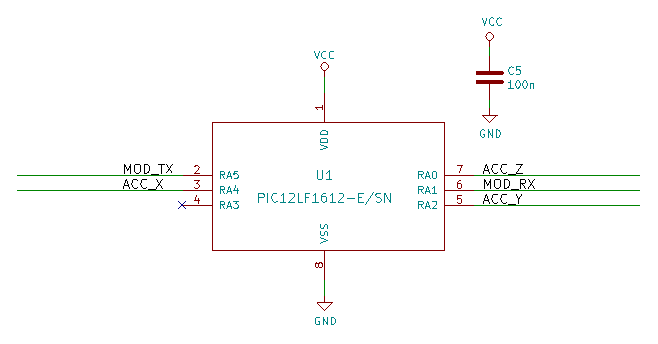
\includegraphics[scale=1.0]{res/schematic-pic.eps}
    \caption{Hardware schematic of the microcontroller}
    \label{fig:sch-pic}
\end{figure}

\subsubsection{Accelerometer}
An accelerometer was connected to the microcontroller to be able to determine the orientation of the tag when held up to a reader.
An analog accelerometer was specifically selected since the PIC12LF1612 lacks serial (SPI/I²C) capability.
The accelerometer MMA7260QT was selected simply due to availability and was connected to the microcontroller through a filtering circuit, as specified in the datasheet\cite{mma-acc}

\begin{figure}[h!]
    \centering
    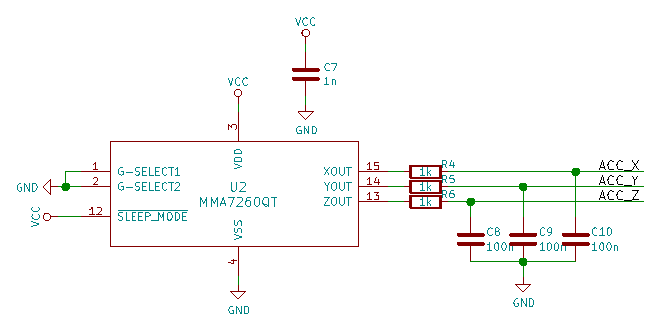
\includegraphics[scale=1.0]{res/schematic-acc.eps}
    \caption{Hardware schematic of the accelerometer}
    \label{fig:sch-acc}
\end{figure}

\subsubsection{Antenna}
The antenna design was based on the field strength detector described in a Ti antenna design application note\cite{ti-antenna}.
The size of the antenna was enlarged to credit-card size and and the number of turns of the antenna coils were reduced from 4 to 3, with the reasoning that it should reduce the inductance, which in turn should make for a lower induced voltage and a higer induced current.
The inductor was realized as a trace on the printed circuit board that was designed for the project.

After the printed circuit board had been created, the inductance of the antenna was measured with and LCR meter.
The measured inductance was 1.0 µH, with a Q-value of 0.008 at 10 kHz.

A tuning capacitor was calculated for the antenna resonant frequency of 13.56 MHz.
At first, 133 pF of capacitance was added (one 100 pF capacitor, one 33 pF capacitor) and a 3 pF - 14 pF adjustable capacitor. The
adjustable capacitor was later replaced with a 10 pF capacitor for a final tuning value of 143 pF.

\begin{figure}[h!]
    \centering
    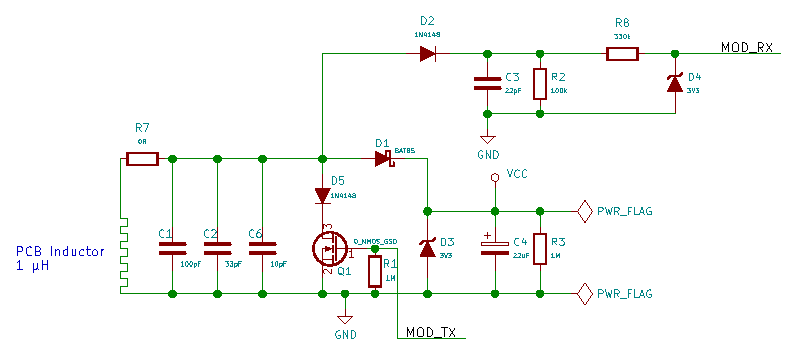
\includegraphics[scale=1.0]{res/schematic-antenna.eps}
    \caption{Hardware schematic of the antenna, modulation and demodulation circuits}
    \label{fig:sch-antenna}
\end{figure}

\begin{figure}[h!]
    \centering
    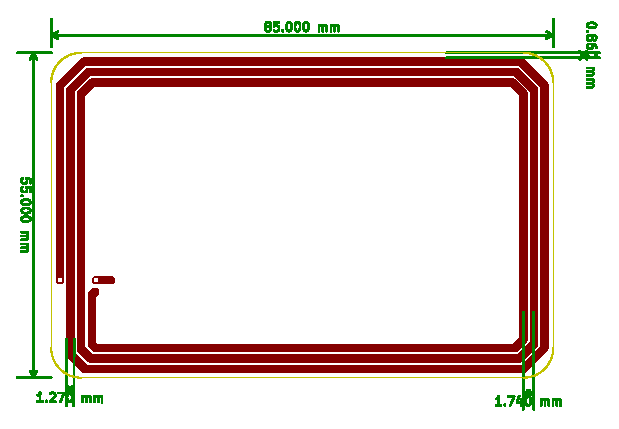
\includegraphics[scale=1.0]{res/softtag-brd-antenna.eps}
    \caption{PCB layout of the antenna inductor}
    \label{fig:brd-antenna}
\end{figure}

\subsubsection{Demodulation Circuitry}
For demodulating the incoming signal, a simple diode-capacitor-resistor based AM detector circuit was selected.
This circuit forms an envelope detector and low pass filter that will filter out the carrier wave and present the modulation wave on the input of the microcontroller.

The filter was initially set around 100 kHz to allow the 10 µs modulation pulses\cite{rfid-iso} through.
This however proved to be inadequate when analysing the signal using an oscilloscope.
The final filter was set around 450 kHz, with component values of 22 pF and 100 kΩ.

A 3.3V zener diode was added to the circuit to protect the microcontroller from high voltages.

\subsubsection{Modulation Circuitry}
For modulating the output signal, a diode in series with an N-channel mosfet, connected across the antenna, was used.

Initially, the diode was not present in the design.
This however caused serious problems, since the body diode of the transistor effectively short-circuited the antenna during half the duty cycle of the carrier wave.
With the diode added, the modulation is only performed during half of the duty cycle of the carrier wave, providing a weaker backscattered signal to the reader but was agreed upon as an acceptable compromise.

The modulation transistor is driven by an output pin of the microcontroller.

\subsubsection{Energy harvester}
The energy harvester was designed as a half-wave rectifier, using a shottky diode.
The shottky diode was selected for its high speed and low forward voltage drop.
High speed is important in the application since the signal being rectified is the carrier wave at 13.56 MHz.
Low forward voltage is important since low power consumption is critical for the application.
Low forward voltage means less energy is wasted in the diode.

A 22 µF tantalum capacitor, a 100 nF ceramic capacitor and a 3.3 V zener diode was added to filter and regulate the voltage supply.

\subsection{Software}
The software implemented in the microcontroller is fairly simple, and is mostly setting up the various built-in
periphials with some very basic flow control. There's three main steps involved, described below.

\subsubsection{Command decoding}
The command decoding that was implemented in the tag is a subset of the standard. Specifically, the
1-in-4 symbol encoding was implemented, as that's what the reader used during testing.

Command decoding is initiated when the comparator (part of the AM detector) triggers an interrupt. Inside the interrupt handler,
a free-running timer is started with the same reset-rate as the symbol rate (1 symbol = 2 bits in 1-in-4 mode)
of the bitstream. A free-running timer was chosen as it is very important to keep the timer in sync with
the transmitter, or drift would eventually lead to corrupted data at the receive end. A hardware
reset on the timer avoid software latency.

If a second pulse within the first symbol arrives at the correct time for a start of frame, the state is
changed from idle to byte recieve mode.

The interrupt is triggered every time the comparator (part of the AM detector) detects a modulated pulse. The interrupt handler then
saves the current counter state. Every time the timer resets, the main loop reads and resets the saved timer
value. The timer value is converted to a 2-byte symbol which is successively shifted into full bytes.

The ISO specification used does specify an end-of-frame symbol. This implementation does not use
the EOF symbol, instead, a symbol with no modulation pulse is used as an EOF marker.
When an end of frame is detected the command is decoded by using the second byte of the received command.
From this byte, a specialized handler function is called, which will parse and encode a result.

\begin{figure}[h!]
    \centering
    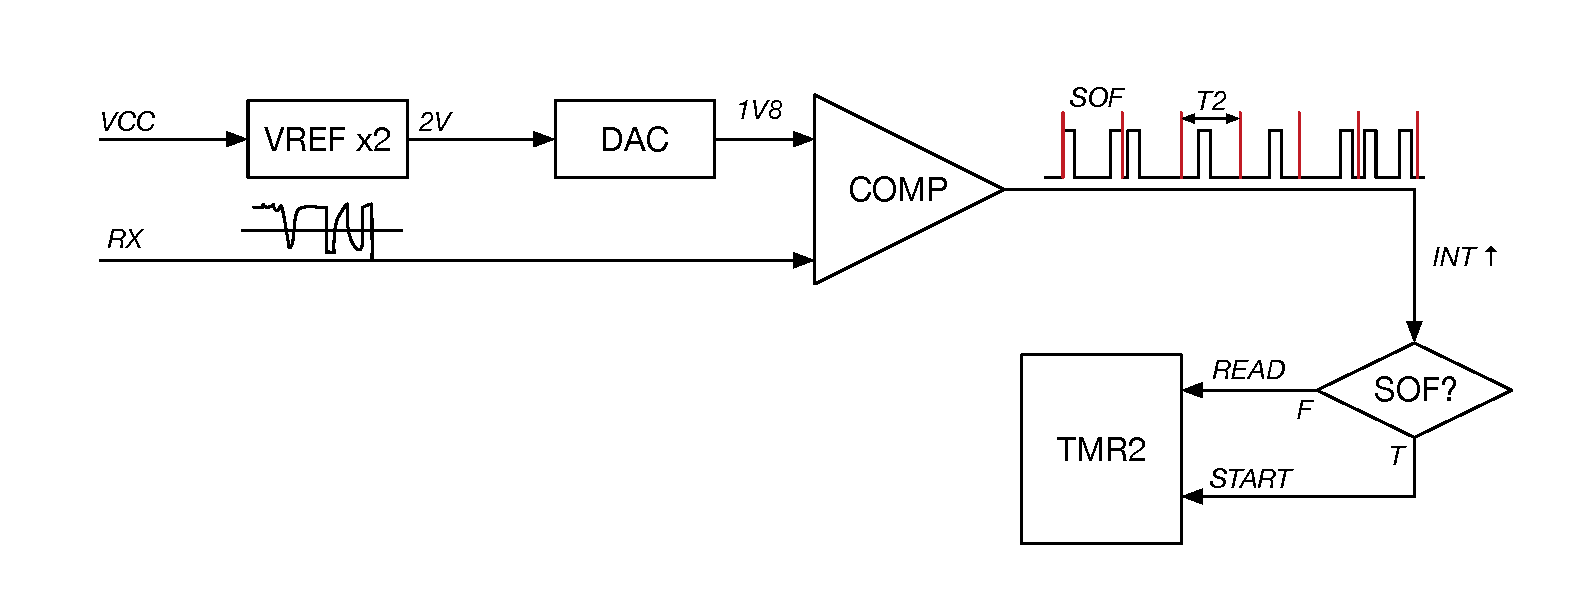
\includegraphics[scale=0.5]{res/RX.pdf}
    \caption{Command decoding in the microcontroller}
    \label{fig:rx}
\end{figure}

\subsubsection{CRC generation}
While CRC (a type of checksum) is designed to be reasonably quick to calculate in software,
a slow microcontroller will still struggle a bit to do it quickly. The microcontroller used in this
tag has a built-in accelerator for CRC computation. On paper, the CRC hardware inside the microcontroller
should be able to do any standard type of CRC up to CRC16, which is good since the ISO standard
implemented for RFID communication calls for a CRC16 checksum in every reply from the tag.

For the most part, configuring the CRC computation accelerator is mainly a case of loading the
CRC polynomial and a half-dozen parameters for things like bit shifting direction, whether or not to pad
out with zeroes when shifting, seed and starting values, which are all given in the ISO standard.
While the shifting direction can be set, the CRC
accelerator does not implement the lowest bit of the CRC polynomial, as any standard polynomial will always have
this bit set. As a result, the CRC accelerator inside the microcontroller cannot do reverse polynomials.
The ISO standard implemented in the tag for RFID communication requires a reverse polynomial CRC.

As a work-around, the polynomial provided by the ISO standard was reversed, and so was the bit shifting
direction as compared to what was called for in the ISO standard. The result is a correctly calculated
CRC, with exception for the bit order, which is completely reversed. A simple work-around for this is to
just shift out the bits in the opposite direction when modulating the reply, or to reverse the bits
in software before transmitting them. The latter is what ended up in the design. Additionally, the ISO standard
calls for the CRC to be transmitted as a one's complement of the calculted CRC, but this operation
can be trivially performed by the microcontroller.


\subsubsection{Response encoding}
The ISO-15693 standard allows for two different ways of transmitting the response: single subcarrier or dual subcarrier.\cite{rfid-iso}
The reader determines which method to use.

It was discovered that the readers in the lab, Texas instrument S6350, requested that the response should use two subcarriers.
This meant that the tag had to be able to generate the frequencies 423.75 kHz and 484.28 kHz, and quickly switch between the two to generate a series of bits that make up the response.

Since the subcarrier frequencies are of fairly high frequency and close together, generating them from the microcontroller proved to be difficult.
Different methods were investigated, including several of the microcontroller's internal peripherals, such as the \emph{Complimentary Waveform Generator} and the \emph{Capture, Compare and PWM} peripheral. External oscillator circuits were also considered, but discarded due to either prohibitive power consumption or cost.

The final solution used the \emph{Capture, Compare and PWM} (CCP) microcontroller peripheral.
Due to restrictions in the microcontroller, the timer peripheral driving the CCP could only run at highest at 8 MHz, toggling the output on each timer compare match.
The closest synthesizable frequencies with this setup are $\frac{\frac{8 MHz}{2}}{8} = 500 kHz$ and $\frac{\frac{8 MHz}{2}}{9} = 444 kHz$.

To solve this problem and generate frequencies closer to the correct subcarrier frequences, the entire microcontroller system oscillator from which all frequencies were derived, was de-tuned.
CCP Dividers of 7 and 8 was chosen instead of 8 and 9 to get the spacing of the subcarriers from eachother correct and the system oscillator was tuned down to the lowest possible setting.
This yielded frequencies of 480.8 kHz and 431 kHz, which was close enough to the standard to work.

\begin{figure}[h!]
    \centering
    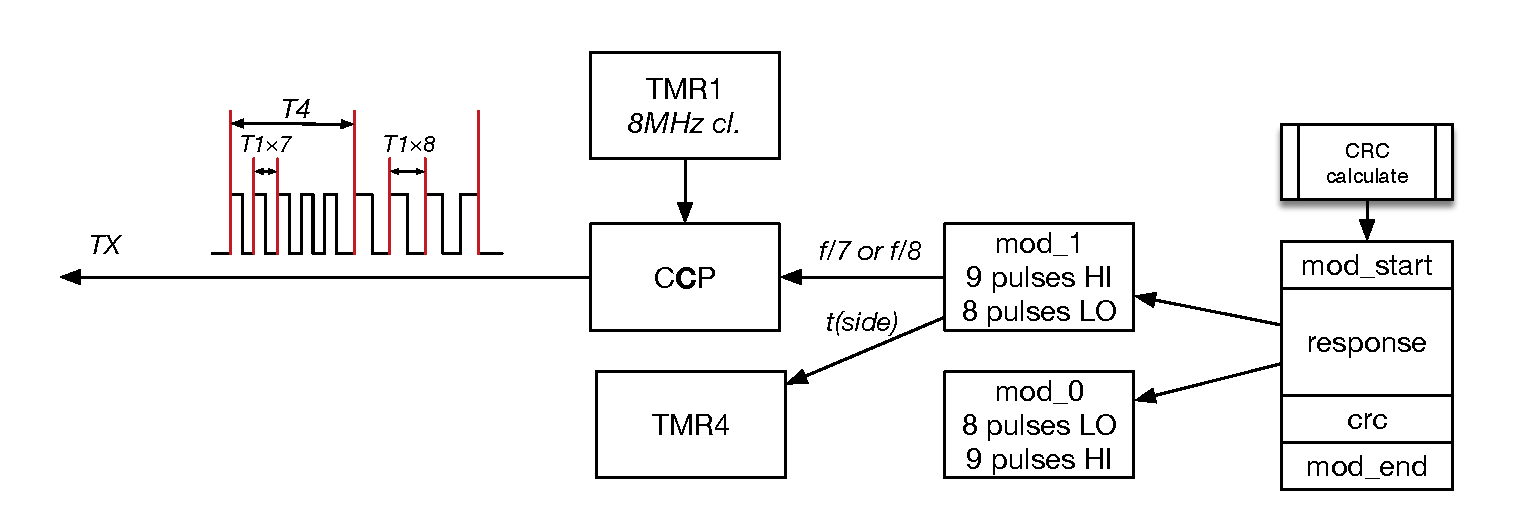
\includegraphics[scale=0.5]{res/TX.pdf}
    \caption{Response encoding in the microcontroller}
    \label{fig:tx}
\end{figure}

%%% Not sure where this should go
%As part of the Inventory command, which is for detecting how many tags are within the reader's range,
%and thier ID numbers, a special collision handling scheme is used. This enables the reader to
%only get replies from certian tags when it thinks multiple tags are replying simultaniously.
%The implementation described in this document does not handle the collision handling fully.
%Specifically, the mask is ignored. Time-slotting is technically not implemented, but as a work-around,
%the lowest 4 bits of the ID was chosen as 0. As a result, the tag will respond in the correct time-slot
%as long as the mask is 0.

%As for the Read Block command, the tag ID field is currently not implemented, the tag will
%reply to any read block command it sees. The address field is however implemented.
%THe Read Block handler will use the address field to select an input for the ADC converter inside
%the microcontrolller. For example, address 0 would be external analog input pin 0, and address 30 would
%be the internal temperature sensor. Whenever a read block command is handled, the corresponding
%analog input is selected and conversion is started. Whenever the ADC has finished converting the analog
%value into a digital one, the data is filled into a response template.
%
%Regardless of command, whenever the data is modulated out, the CRC is first calculated as per the section
%below. The reply is kept in a buffer in RAM. However, due to timing concerns, there is one transmit function per
%response length, containing only an unrolled loop with calls to helpers that m
